% At least, use document class book
\documentclass[a4paper]{article}

\usepackage[T1]{fontenc}
\usepackage[latin1]{inputenc}
\usepackage{listings}
\usepackage{graphicx}
\usepackage{eso-pic}
\usepackage{pstricks}
\usepackage{listings}
\usepackage{graphicx}

\usepackage{color}
\definecolor{darkgreen}{rgb}{0,0.5,0}

% F�r listings
\usepackage{listings}
\lstset{
  frame=single,
  frameround=tttt,
  xleftmargin=0.7cm,
  xrightmargin=0.3cm,
  numbers=left,
  basicstyle=\fontfamily{pcr} \small \color{black},
  keywordstyle=\bfseries \color{blue},
	stringstyle=\color{red},
	commentstyle=\color{darkgreen},
	breaklines=true,
	showstringspaces=false
}

% F�r Metadaten im PDF.
\usepackage[
  bookmarksnumbered=true,
  pdftitle={How to use the Java Code Generator Ocl2Java},
  pdfauthor={Claas Wilke},
  pdfcreator={TeXnicCenter},
  pdfkeywords={OCL, Dresden OCL, constraints, Java, AspectJ, code, generation, instrumentation},
  pdfsubject={A Tutorial which describes how the Java Code Generator of Dresden OCL2 for Eclipse can be used.}
]{hyperref}
\definecolor{LinkColor}{rgb}{0,0,1}
	
\hypersetup{
  colorlinks=true,
  linkcolor=LinkColor,
  citecolor=LinkColor,
  filecolor=LinkColor,
  menucolor=LinkColor,
  urlcolor=LinkColor
} 

\newcommand{\reference}[1]{{\begin{ttfamily}#1\end{ttfamily}}}

\newcommand{\model}[1]{{\begin{ttfamily}#1\end{ttfamily}}}
\newcommand{\eclipse}[1]{{\begin{itshape}#1\end{itshape}}}


\begin{document}

% Define the title of the thesis
\title{How to use the Java Code Generator Ocl2Java}
% Specify the author of the thesis
\author{Claas Wilke}
% Specify the date on which the thesis is handed in

\maketitle

This tutorial describes how the Java Code Generator \textit{Ocl2Java} provided with \textit{Dresden OCL2 for Eclipse} can be used. A general introduction into \textit{Dresden OCL2 for Eclipse} can be found in \cite{tut:general}. A detailed documentation of the development of \textit{Ocl2Java} can be found in \cite{GB:Wilke}.

The procedure described in this tutorial was realized and tested with \textit{Eclipse 3.4.1} \cite{Ecl}. In addition to that this tutorial should also run with \textit{Eclipse 3.3.x}. Besides \textit{Eclipse} you also need to install some required plug-ins. Table \ref{tab:software} shows all required software to run \textit{Dresden OCL2 for Eclipse} and \textit{Ocl2Java}.
  
\begin{figure}[!htbp]
\begin{tabular}[h]{|p{5.2cm}|p{6cm}|}
    \hline
    \textbf{Software} & \textbf{Available at} \\
    \hline
    Eclipse 3.4.x & http://www.eclipse.org/ \\
    \hline
    Eclipse Modeling Framework\newline (EMF) & http://www.eclipse.org/modeling/emf/ \\
    \hline
    AspectJ Development Tools\newline (AJDT) (only to run\newline the generated code) & http://www.eclipse.org/aspectj/ \\
    \hline
    Eclipse Model Development Tools\newline (MDT) (only with the UML2.0\newline meta model) & http://www.eclipse.org/modeling/mdt/ \\
    \hline
    Eclipse Plugin Development\newline Environment (only to run the\newline toolkit using the source code\newline distribution) & http://www.eclipse.org/pde/ \\
    \hline
\end{tabular}
\caption{Software needed to run \textit{Dresden OCL2 for Eclipse} and \textit{Ocl2Java}.}
\label{tab:software}
\end{figure}


	
\section{How to run Dresden OCL2 for Eclipse}

How to run the toolkit \textit{Dresden OCL2 for Eclipse} and how to load models and OCL constraints will not be explained in this tutorial. This tutorial assumes that the user is familiar with such basic use of the toolkit. A general introduction into \textit{Dresden OCL2 for Eclipse} can be found in \cite{tut:general}.




\section{The example used during this tutorial}

This tutorial uses the \textit{Simple Example} which is provided with \textit{Dresden OCL2 for Eclipse} located in the plug-in package \reference{tudresden.ocl20.pivot.examples.\linebreak[0]simple}. An overview over all examples provided with \textit{Dresden OCL2 for Eclipse} can be found in \cite{tut:examples}. Figure \ref{pic:Simple} shows the class structure which is described by the \textit{Simple Example}. 

\begin{figure}[!htbp]
	\centering
	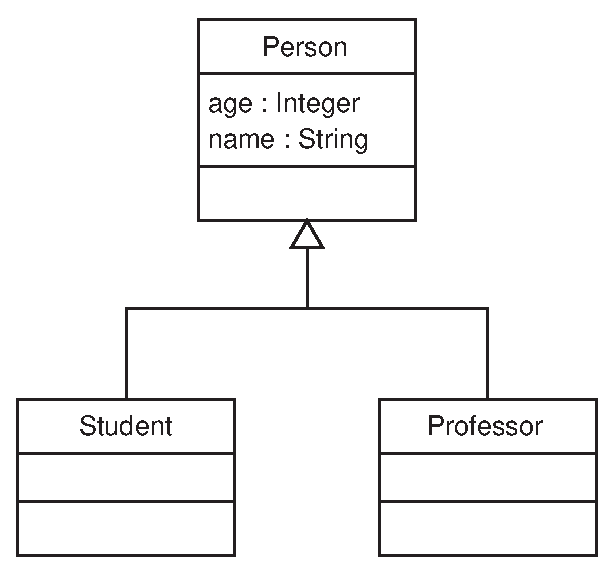
\includegraphics[width=0.5\linewidth]{figures/simpleExample}
	\caption{The class diagram described by the simple example model.}
	\label{pic:Simple}
\end{figure}

The model of the example defines three classes: The class \model{Person} has two attributes \model{age} and \model{name}. Two subclasses of \model{Person} are defined, \model{Student} and \model{Professor}.

To import the \textit{Simple Example} into our Eclipse workspace we create a new Java project into our Workspace called \model{tudresden.ocl20.pivot.examples.\linebreak[0]simple} and use the import wizard \eclipse{General -> Archive File} to import the example provided as jar archive. In the following window we select the directory were the jar file is located (eventually the \model{plugins} directory into the Eclipse root folder) and we select the archive \model{tudresden.ocl20.pivot.examples.simple.\linebreak[0]jar} and click the \eclipse{Finish} button (if you use a source code distribution of \textit{Dresden OCL2 for Eclipse} instead, you can simple import the project \model{tudresden.ocl20.\linebreak[0]pivot.examples.simple} using the import wizard \eclipse{General -> Existing Projects into Workspace}).

Next, we have to import a second project called \model{tudresden.ocl20.pivot.\linebreak[0]examples.simple.constraints}. We can use the same mechanism explained above, but instead of a Java project we now create an AspectJ project before we import the archive file (if the wizard to create an AspectJ project is not available you have to install the \textit{AspectJ Development Tools} first). Figure \ref{pic:packageExplorer} shows the package Explorer containing both imported projects.

\begin{figure}[!htbp]
	\centering
	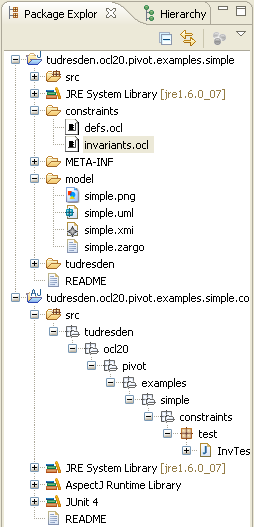
\includegraphics[width=0.5\linewidth]{figures/packageExplorer}
	\caption{The package explorer containing the two projects which are needed to run this tutorial.}
	\label{pic:packageExplorer}
\end{figure}

Now we have imported all files we need to run this tutorial. The first project provides a model file which contains the simple class diagram which has been explained above (the model file is located at \model{model/simple.uml}) and the constraint file we want to generate code for (the constraint file is located at \model{constraints/invariants.ocl}). Listing \ref{simpleInvariant} shows one invariant which is contained in the constraint file for which we want to generate code. For this invariant which denotes, that the \model{age} of any \model{Person} must be greater or equal to zero at any time during the life cycle of the \model{Person}.

\lstset{
  language=OCL
}
\begin{lstlisting}[caption={A simple invariant.}, captionpos=b, label=simpleInvariant, float]
-- The age of Person can not be negative.
context Person
inv: age >= 0
\end{lstlisting}

The second project provides a class \model{src/tudresden.ocl20.pivot.examp\-les.simple.constraints.InvTest.java}\linebreak[0] which contains a jUnit test case which checks, whether or not the mentioned constraint is enforced by generated code. The test case creates two \model{Persons} and tries to set their \model{age}. The \model{age} of the second \model{Person} is set to \model{-3} and thus the constraint is violated. The test case expects that a runtime exception is thrown, when the constraint is violated.

The code for the mentioned constraint has not been generated yet and thus the exception will not be thrown. We run the test case by right clicking on the Java class in the \eclipse{Package Explorer} and selecting the menu item \eclipse{Run as -> JUnit Test}. The test case fails because the exception is not thrown (see figure \ref{pic:junit1}). To fulfill the test case we have to generate the ApsectJ code for the constraint which enforces the constraint's condition. How to create such code will be explained in the following.

\begin{figure}[!htbp]
	\centering
	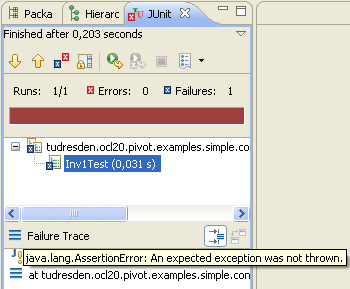
\includegraphics[width=0.6\linewidth]{figures/junit1}
	\caption{The result of the jUnit test case.}
	\label{pic:junit1}
\end{figure}




\section{Prepare the Code Generation}

To prepare the code generation we have to import the model \model{model/simple.uml} into the \eclipse{Model Browser}. We use the import wizard for domain specific models of the toolkit to import the model. This procedure is explained in the already mentioned general tutorial (\cite{tut:general}). Then we have to import the constraint file \model{constraints/invariant.ocl} which is done by an import wizard again. Afterwards, the model explorer should look like illustrated in figure \ref{pic:modelBrowser}. Now we can start the code generation.

\begin{figure}[!htbp]
	\centering
	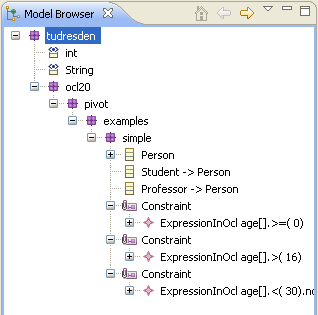
\includegraphics[width=0.6\linewidth]{figures/modelBrowser}
	\caption{The model browser containing the simple model and its constraints.}
	\label{pic:modelBrowser}
\end{figure}




\section{The Code Generation}

To start the code generation we click on the menu item \eclipse{DresdenOCL} and select the item \eclipse{Generate AspectJ Constraint Code}. 


\subsection{Selecting a Model}

A wizard opens and we have to select a model for code generation (see figure \ref{pic:wizard1}). We select the \model{simple.uml} model and click the \eclipse{Next} button.

\begin{figure}[!htbp]
	\centering
	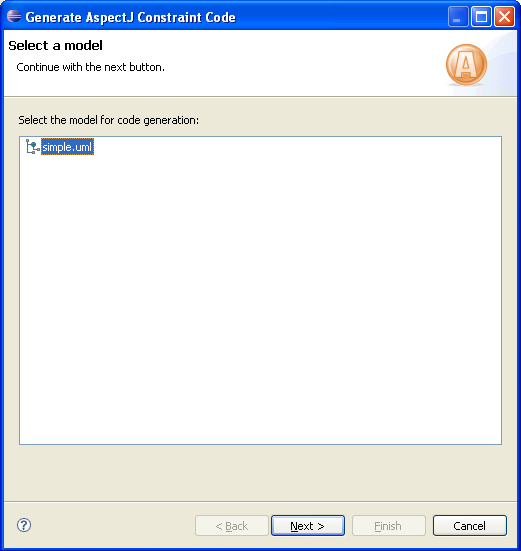
\includegraphics[width=1.0\linewidth]{figures/wizard1}
	\caption{The first step: Selecting a model for code generation.}
	\label{pic:wizard1}
\end{figure}


\subsection{Selecting Constraints}

As a second step we now have to select the constraints for which we want to generate code. We only select the constraint which enforce that the \model{age} of any \model{Person} must be equal to or greater than zero and click the \eclipse{Next} button (see figure \ref{pic:wizard2}).

\begin{figure}[!htbp]
	\centering
	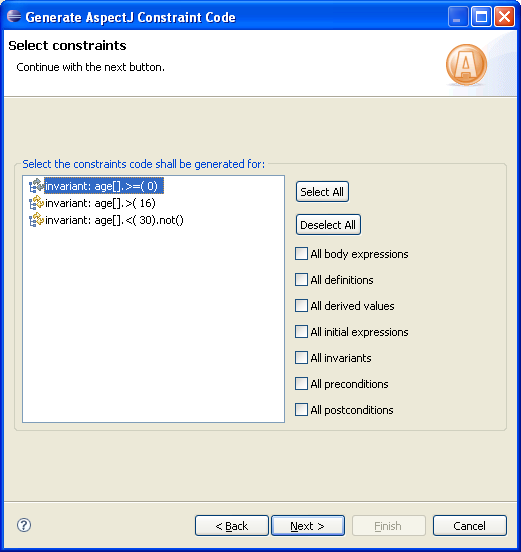
\includegraphics[width=1.0\linewidth]{figures/wizard2}
	\caption{The second step: Selecting constraints for code generation.}
	\label{pic:wizard2}
\end{figure}


\subsection{Selecting a Target Directory}

Next, we have to select a target directory to which our code shall be generated. We select the source directory of our second project (which is \model{tudresden.\linebreak[0]ocl20.pivot.examples.simple.constraints/src}) (see figure \ref{pic:wizard3}). Please note, that we select the source directory and not the package directory into which the code shall be generated! The code generator creates or uses contained package directories depending on the package structure of the selected constraint. Additionally we can specify a sub folder into which the constraint code shall be generated relatively to the package of the constrained class. By standard this is a sub directory called \model{constraints}. We don't want to change this setting and click the \eclipse{Next} button.
	
\begin{figure}[!htbp]
	\centering
	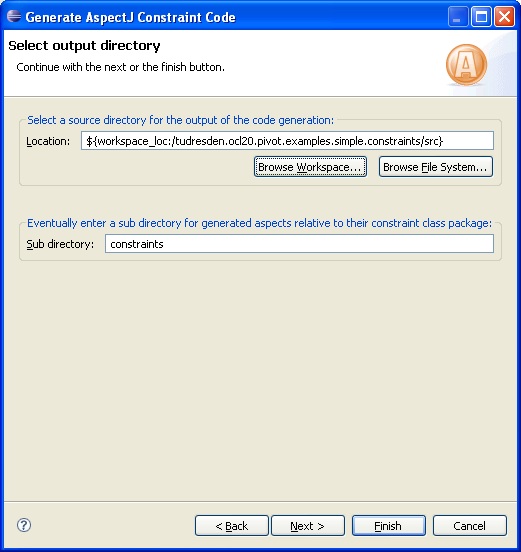
\includegraphics[width=1.0\linewidth]{figures/wizard3}
	\caption{The third step: Selecting a target directory for the generated code.}
	\label{pic:wizard3}
\end{figure}


\subsection{Specifying General Settings}
	
On the following page of the wizard we can specify general settings for the code generation (see figure \ref{pic:wizard4}).

\begin{figure}[!htbp]
	\centering
	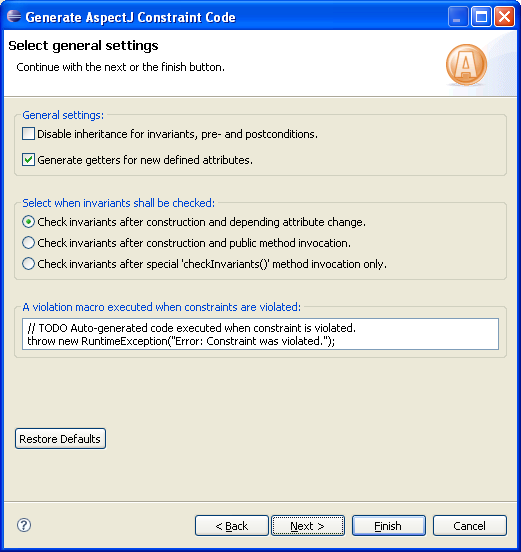
\includegraphics[width=1.0\linewidth]{figures/wizard4}
	\caption{The fourth step: General settings for the code generation.}
	\label{pic:wizard4}
\end{figure}

\begin{figure}[!htbp]
	\centering
	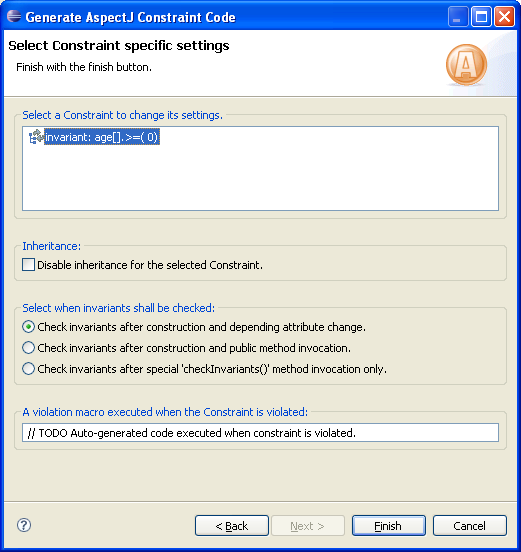
\includegraphics[width=1.0\linewidth]{figures/wizard5}
	\caption{The fifth step: Constraint specific settings for the code generation.}
	\label{pic:wizard5}
\end{figure}

We can disable the inheritance of constraints (which would not be useful in our example because we want to enforce the constraint for \model{Persons}, but for \model{Students} and \model{Professors} as well). We can also enable that the code generator will generate getter methods for new defined attributes of \model{def} constraints.

More interesting is the possibility to select one of three provided strategies, when invariants shall be checked during runtime:

\begin{enumerate}
	\item Invariants can be checked after construction of an object and after any change of an attribute or association which is in scope of the invariant condition (\textit{Strong Verification}).
	\item Invariants can be checked after construction of an object and before or after the execution of any public method of the constrained class (\textit{Weak Verification}).
	\item And finally, invariants can only be checked if the user calls a special method at runtime (\textit{Transactional Verification}).
\end{enumerate}

This three scenarios can be useful for users in different situations. If a user wants to verify strongly, that his constraints are verified after any change of any dependent attribute he should use \textit{strong verification}. If he wants to use attributes to temporary store values and constraints shall only be verified if any external class instance wants to access values of the constrained class, he should use \textit{weak verification}. If the user wants to work with databases or other remote communication and the state of his constraint classes should be only valid before data transmission, he should use the scenario \textit{transactional verification}.

Finally, we can specify a \textit{violation macro} which specifies the code, which will be executed when a constraint is violated during runtime. By default, the \textit{violation macro} throws a runtime exception. We also want to have a runtime exception thrown when our constraint is violated. Thus, we don't change the \textit{violation macro} and continue with the \eclipse{Next} button.


\subsection{Constraint Specific Settings}

The last page of the code generation wizard provides the possibility to configure some of the code generation settings constraint specific by selecting a constraint and adapting it's settings (see figure \ref{pic:wizard5}). We don't want to adapt the settings, thus we can finish the wizard and start the code generation by clicking the \eclipse{Finish} button.




\section{The Generated Code}

After finishing the wizard, the code for the selected constraint will be generated. To see the result, we have to refresh our project in the workspace. We select the project \model{tudresden.ocl20.pivot.examples.simple.constraint} in the \eclipse{Package Explorer} open the context menu with a right mouse click and select the menu item \eclipse{Refresh}. Afterwards, our project contains a new generated AspectJ file called \model{tudresden.ocl20.pivot.examples.simple.constraints.InvAspect\-01.aj} (see figure \ref{pic:packageExplorer2}).
	
\begin{figure}[!htbp]
	\centering
	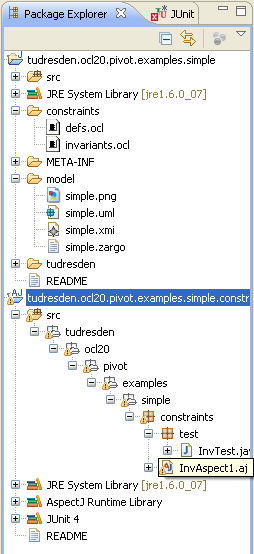
\includegraphics[width=0.5\linewidth]{figures/packageExplorer2}
	\caption{The package explorer containing the new generated aspect file.}
	\label{pic:packageExplorer2}
\end{figure}

Now we can rerun our jUnit test case. The test case finishes successfully because the expected runtime exception is thrown (see figure \ref{pic:junit2}).	

\begin{figure}[!htbp]
	\centering
	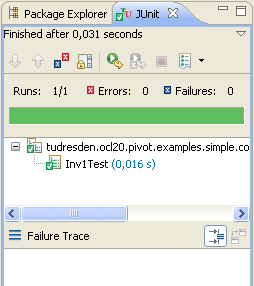
\includegraphics[width=0.5\linewidth]{figures/junit2}
	\caption{The successfully finished jUnit test case.}
	\label{pic:junit2}
\end{figure}


	
	
\section{Conclusion}
  
This tutorial described how to generate AspectJ code using the \textit{Ocl2Java} code generator of \textit{Dresden OCL2 for Eclipse}. More information about \textit{Dresden OCL2 for Eclipse} is available at the website of the \textit{Dresden OCL Toolkit} \cite{ToolkitHP}.




\newpage
\bibliographystyle{alphadin}
\bibliography{ocl2java}
% Literaturliste in Inhalt aufnehmen.
\addcontentsline{toc}{section}{References}




\end{document}
